%; whizzy chapter
% -initex iniptex -latex platex -format platex -bibtex jbibtex -fmt fmt
% 以上 whizzytex を使用する場合の設定。

%     Kansai Debian Meeting resources
%     Copyright (C) 2007 Takaya Yamashita
%     Thank you for Tokyo Debian Meeting resources

%     This program is free software; you can redistribute it and/or modify
%     it under the terms of the GNU General Public License as published by
%     the Free Software Foundation; either version 2 of the License, or
%     (at your option) any later version.

%     This program is distributed in the hope that it will be useful,
%     but WITHOUT ANY WARRANTY; without even the implied warranty of
%     MERCHANTABILITY or FITNESS FOR A PARTICULAR PURPOSE.  See the
%     GNU General Public License for more details.

%     You should have received a copy of the GNU General Public License
%     along with this program; if not, write to the Free Software
%     Foundation, Inc., 51 Franklin St, Fifth Floor, Boston, MA  02110-1301 USA

%  preview (shell-command (concat "evince " (replace-regexp-in-string "tex$" "pdf"(buffer-file-name)) "&"))
% 画像ファイルを処理するためにはebbを利用してboundingboxを作成。
%(shell-command "cd image200708; ebb *.png")

%%ここからヘッダ開始。

\documentclass[mingoth,a4paper]{jsarticle}
\usepackage{kansaimonthlyreport}
\usepackage[dvips]{xy}

% 日付を定義する、毎月変わります。
\newcommand{\debmtgyear}{2009}
\newcommand{\debmtgdate}{27}
\newcommand{\debmtgmonth}{09}
\newcommand{\debmtgnumber}{27}

\begin{document}

\begin{titlepage}

% 毎月変更する部分、本文の末尾も修正することをわすれずに

 第\debmtgnumber{}回 関西 Debian 勉強会資料

\vspace{2cm}

\begin{center}

\includegraphics{image200802/kansaidebianlogo.png}
\end{center}

\begin{flushright}
\hfill{}関西 Debian 勉強会担当者 のがた・倉敷・佐々木\\
\hfill{}\debmtgyear{}年\debmtgmonth{}月\debmtgdate{}日
\end{flushright}

\thispagestyle{empty}
\end{titlepage}

\dancersection{Introduction}{Debian JP}
 
 関西 Debian 勉強会はDebian GNU/Linux のさまざ
 まなトピック(新しいパッケージ、Debian 特有の機能の仕組、Debian 界隈で起
 こった出来事、などなど)について話し合う会です。

 目的として次の三つを考えています。
 \begin{itemize}
  \item MLや掲示板ではなく、直接顔を合わせる事での情報交換の促進
  \item 定期的に集まれる場所
  \item 資料の作成
 \end{itemize}

 それでは、楽しいひとときをお過ごし下さい。

\newpage

\begin{minipage}[b]{0.2\hsize}
 {\rotatebox{90}{\fontsize{80}{80}
{\gt 関西デビアン勉強会}}}
\end{minipage}
\begin{minipage}[b]{0.8\hsize}
\hrule
\vspace{2mm}
\hrule
\setcounter{tocdepth}{1}
\tableofcontents
\vspace{2mm}
\hrule
\end{minipage}

%-------------------------------
\dancersection{最近の Debian 関係のイベント報告}{Debian JP}

\subsection{前回の関西 Debian 勉強会}

8月23日に、福島区民センターにて開催されました。内容は、lintian を
使ったパッケージチェック方法の解説と、DDTSS を使ったパッケージ説明
文翻訳のハンズオンを行いました。


\subsection{東京でのキーサインパーティー}

9月16日に、東京エリアの勉強会としてキーサインパーティーが開催されました。
Debian 開発者が 8 名も参加する勢いで、大変盛況だったようです。

最近、矢吹さんも Debian 開発者になられましたので、関西でも近いうちに
企画したいところですね。ちなみに、強度を上げた gpg 鍵の作成方法は、
ささきさんの blog に記事がありますので参照してみてください。

%-------------------------------
\dancersection{GUIがついて格好良くなったreportbugを使ってみよう}{のがたじゅん}

\subsection{はじめに}

Debianのバグ報告支援ツールreportbugが、バージョン3.99.0からGTK2を利用した
ユーザーインターフェースが使えるようになっていましたが、あまり知られていない
のでreportbugの使い方も兼ねて書いてみました。

\subsubsection{おわび}

「使ってみよう」とタイトルに書きましたが、実際にGTK2インターフェースで使
うとquerybtsがうまく動かず登録されたバグを表示することができなかったり、
戻るボタンで戻ると入力ができなかったりと不具合あります。ですので「使う」
には難しいところもありますが、とりあえずこんな感じということを知ってもら
えれば思います。

\subsection{reportbugとは}

Debianを使っていて発見したバグは、決められた書式にしたがって書いたメール
をDebianのバグ追跡システム(Bug Tracking System.通称BTS)に送ることによって
バグを報告することができます \footnote{バグレポートから参加するDebianパッ
ケージ開発 / 木下 達也 (あんどきゅめんてっど でびあん 2008年夏号)

\url{http://tokyodebian.alioth.debian.org/pdf/debianmeetingresume2008-natsu.pdf}}。ですがバグ報告に慣れていないと、決められた
書式でメールを書くことはもちろんのこと、バグ修正に必要なパッケージ情報な
どを洩れなく集めたりすることは大変なことです。

reportbugは、そういったバグ報告の負担を減らすためのツールで、バグ検索から、
バグ報告のためのパッケージ情報の収集、バグ登録に必要なメールの書式整形、
報告メールの送信まで行ってくれるツールです。

\subsection{reportbugのインストール}

Debianインストール時に「標準システム」を選択すると、reportbugはインストー
ルされますが、GTK2や端末上でのメニューインターフェースに必要なRecommends
やSuggestsパッケージはインストールされないので、改めてreportbugをインストー
ルします。

\begin{commandline}
 # apt-get update
 # apt-get remove reportbug
 # apt-get -o APT::Install-Suggests=true --install-recommends -y install reportbug
\end{commandline}

まどろっこしいことをしていますが、すでにインストールされたパッケージの
RecommendsやSuggestsパッケージをスマートにインストールするにはどうしたら
いんでしょうか?

\subsection{reportbugを起動}

reportbugを起動します。

デスクトップのメニュー([アプリケーション]→[システムメ
ニュー]→[reportbug])から起動すると、GTK2インターフェースのウィンドウが開
きます。端末から起動するとメッセージが表示されます。

\begin{commandline}
 $ reportbug 
\end{commandline}

\begin{figure}[h]
 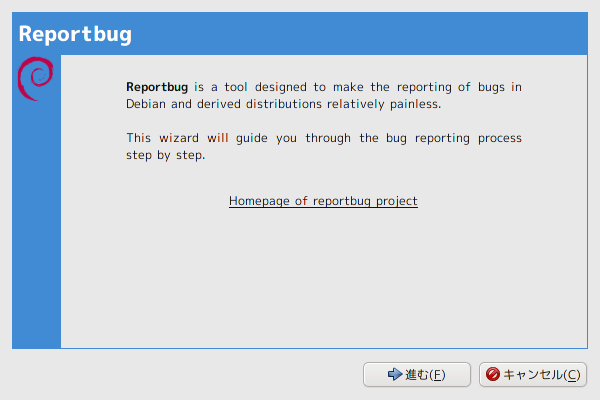
\includegraphics[scale=0.5]{image200909/reportbug-initial.png}
 \caption[reportbugのGTK2インターフェース]{reportbugのGTK2インターフェース}
\end{figure}

\subsection{初期設定}
reportbugを初めて起動すると、reportbugを使うための設定を尋ねられます。
初期設定の途中、バグ報告メールを送信するためのメール環境について尋ねられ
るので、あらかじめメールの設定を確認しておいてください。
設定例では、Gmailを使っていることを前提に話を進めます。

\begin{itemize}
 \item 参考: その他のメール クライアントの設定 - Gmail ヘルプ:

\url{http://mail.google.com/support/bin/answer.py?hl=jp&answer=13287}
\end{itemize}

\begin{commandline}
Welcome to reportbug! Since it looks like this is the first time you have used reportbug, we are configuring its behavior.

These settings will be saved to the file "/home/hoge/.reportbugrc", which you will be free to edit further.                
Please choose the default operating mode for reportbug.                                                                   

1 novice    Offer simple prompts, bypassing technical questions.

2 standard  Offer more extensive prompts, including asking about things that a moderately sophisticated user would be
            expected to know about Debian.                                                                           

3 advanced  Like standard, but assumes you know a bit more about Debian, including "incoming".

4 expert    Bypass most handholding measures and preliminary triage routines. This mode should not be used by people
            unfamiliar with Debian's policies and operating procedures.                                             

Select mode: [novice] 
\end{commandline}

ウェルカムメッセージと設定は~/.reportbugrcに保存されていますと二つのお知
らせの後、reportbugで使うモードについて尋ねています。とりあえずは細かいこ
とよりバグ報告だけに絞りたいので、noviceのままでよいでしょう。

\newpage

\begin{commandline}
Please choose the default interface for reportbug.

1 text   A text-oriented console user interface

2 gtk2   A graphical (GTK+) user interface.

3 urwid  A menu-based console user interface

Select interface: 2
\end{commandline}

どのユーザーインターフェースを使うか選択します。
今回はテーマにそってgtk2を選びました。実際に使うとなるとurwidが使いやす
いと思います。

\begin{commandline}
Will reportbug often have direct Internet access? (You should answer yes to this question unless you know what you are doing
and plan to check whether duplicate reports have been filed via some other channel.) [Y|n|q|?]?
\end{commandline}

インターネットに接続しているかですが、おそらくほとんどの人は接続している
と思うので、yと答えます。

\begin{commandline}
What real name should be used for sending bug reports?
[Hogewo HOGETA]>
\end{commandline}

バグ報告に使う名前を設定します。

\begin{commandline}
Which of your email addresses should be used when sending bug reports? (Note that this address will be visible in the bug
tracking system, so you may want to use a webmail address or another address with good spam filtering capabilities.)
[example@gmail.com]>
\end{commandline}

バグ報告に使うメールアドレスを設定します。
ここで気をつけないといけないことは、ここで設定したメールアドレスはバグ報
告をすると公開されます。あまり公開したくないメールアドレスは設定しないほ
うがよいでしょう。

\begin{commandline}
Do you have a "mail transport agent" (MTA) like Exim, Postfix or SSMTP configured on this computer to send mail to the
Internet? [Y|n|q|?]? n
\end{commandline}

バグ報告をするマシンでメールサーバーが動いているか尋ねています。
GmailのSMTPサーバーを使って送信するので、ここではnと答えます。

\begin{commandline}
Please enter the name of your SMTP host.  Usually it's called something
 like "mail.example.org" or "smtp.example.org".
If you need to use a different port than default, use the <host>:<port> alternative format.

Just press ENTER if you don't have one or don't know.
> smtp.gmail.com:587
\end{commandline}

送信するSMTPサーバーを登録します。
GmailのSMTPサーバーのアドレスはsmtp.gmail.com、ポート番号は587なので、
smtp.gmail.com:587と登録します。

\begin{commandline}
If you need to use a user name to send email via "smtp.gmail.com:587" on your computer, please enter that user name. Just
press ENTER if you don't need a user name.
> nogajun@gmail.com
\end{commandline}

SMTPサーバーを利用するためのユーザー名を登録します。
GmailのSMTPサーバーを使うにはドメイン名も含めたユーザー名が必要なので、<ユーザー
名>@gmail.comと登録します。

\begin{commandline}
Does your SMTP host require TLS authentication? [y|N|q|?]? y
\end{commandline}

SMTPはTLSを使うかの問いについては、Gmailでは必要なのでyと答えます。

\begin{commandline}
Please enter the name of your proxy server. It should only use this parameter if you are behind a firewall. The PROXY
argument should be formatted as a valid HTTP URL, including (if necessary) a port number; for example,
http://192.168.1.1:3128/. Just press ENTER if you don't have one or don't know.
>
\end{commandline}
Proxyについて尋ねています。使っていれば設定します。使っていなければ空のまま
でEnterキーを押します。

\begin{commandline}
Default preferences file written. To reconfigure, re-run reportbug with the "--configure" option.
\end{commandline}
初期設定が終わりました。もう一度、設定をやり直したいときは、--configureオ
プションをつけて起動するとやり直すことができます。

\subsection{reportbugを使ってみる}

 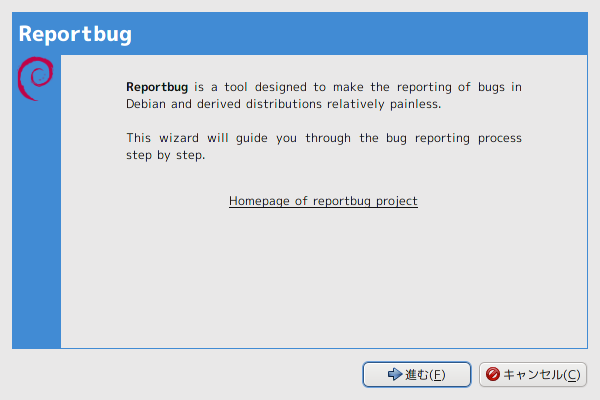
\includegraphics[scale=0.5]{image200909/reportbug-1.png}

起動するとこんな感じです。ウィザード形式なのでわかりやすいと思います。

 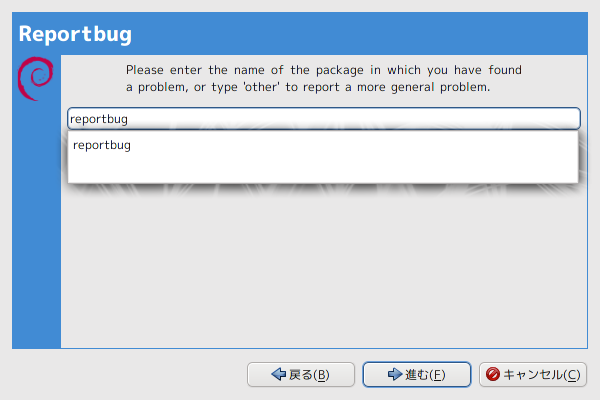
\includegraphics[scale=0.5]{image200909/reportbug-2.png}

バグを見つけたパッケージ名を入力します。パッケージ名の頭を何文字か入力す
ると、インストールされているパッケージの候補を表示してくれます。

 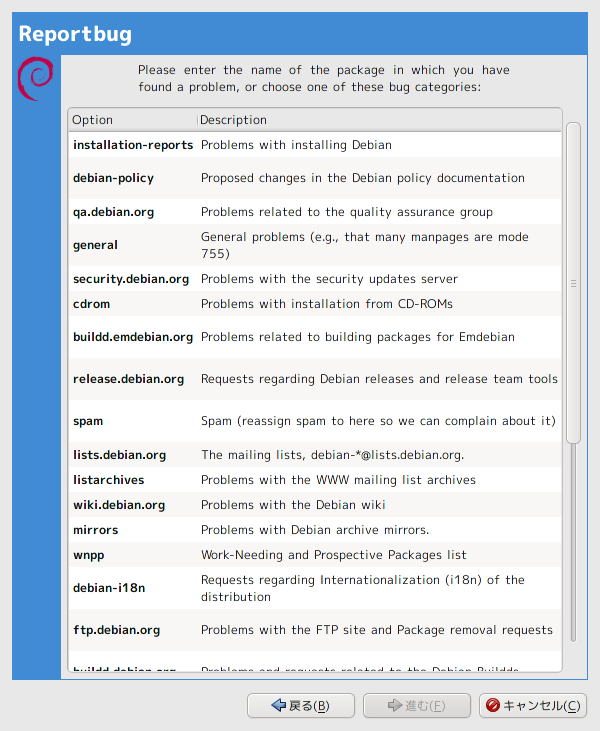
\includegraphics[scale=0.5]{image200909/reportbug-8.png}

パッケージ名の入力でotherと入力するとこの画面になります。これは擬似パッケー
ジの一覧です。パッケージ以外に見つけたDebianに関連する問題を擬似パッケー
ジのバグとして登録します。

\begin{itemize}
 \item Debian -- Debian バグ追跡システム - 擬似パッケージ:

\url{http://www.debian.org/Bugs/pseudo-packages.ja.html}

\end{itemize}

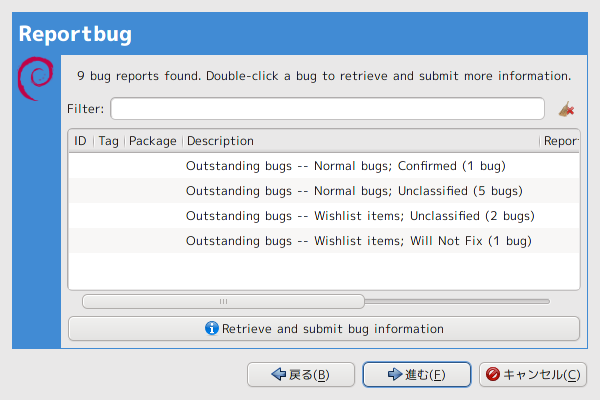
\includegraphics[scale=0.5]{image200909/reportbug-3.png}

本来ならばここに登録されたバグが表示されて、今から登録しようとしたバグが
すでに登録済みかどうか確認できるのですが、GTK2インターフェースだと
querybtsがうまく動かなくて(\#432178)、ダブルクリックをしても何も表示され
ません。残念。

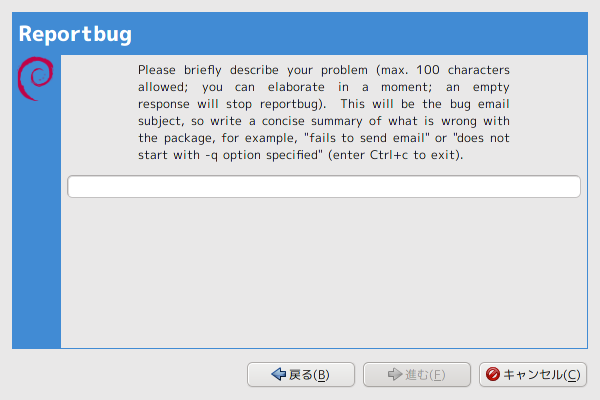
\includegraphics[scale=0.5]{image200909/reportbug-4.png}

バグがまだ登録されていなかったとして次に進むと、バグを登録する画面に入り
ます。ここではバグの概要を簡潔に書きます。

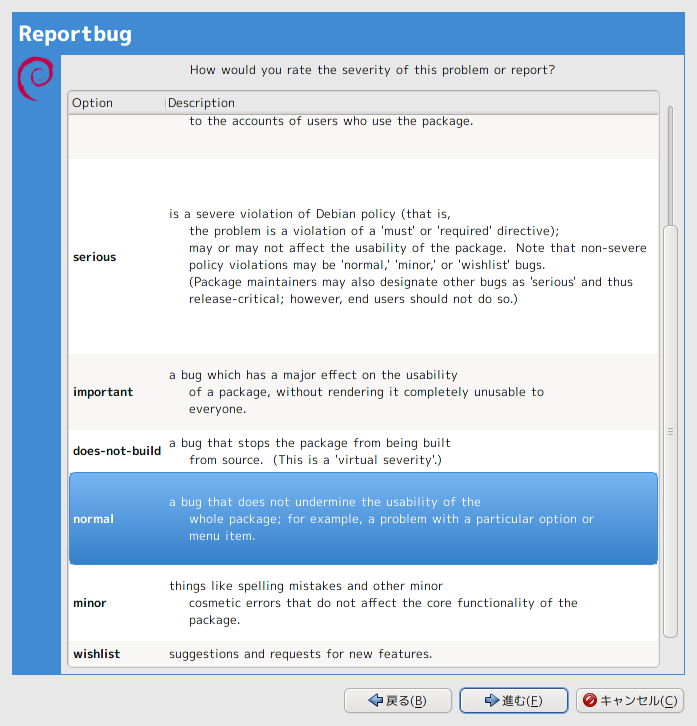
\includegraphics[scale=0.5]{image200909/reportbug-5.png}

バグの種類を指定します。種類はCriticalやSeriousのような深刻なものから、提
案のWhishlistまであります。通常はnormalでいいと思います。

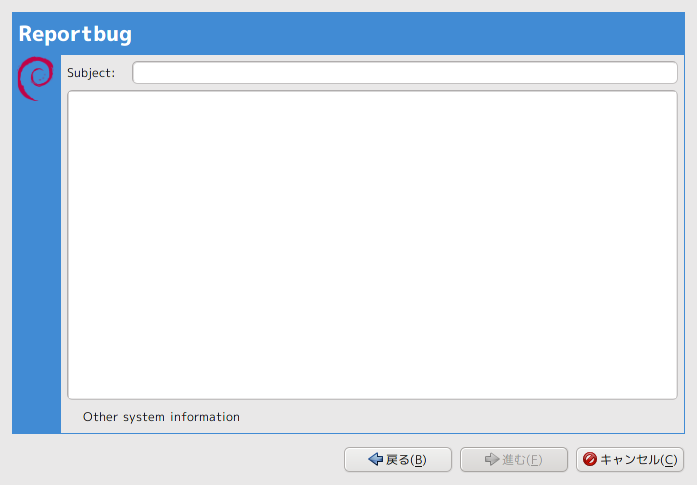
\includegraphics[scale=0.5]{image200909/reportbug-6.png}

ここでは、バグの内容を書きます。
スクリーンショットのために適当なことを書いて撮っていたのでSubjectは消して
いますが、通常はSubjectの箇所に上で書いたバグの概要が入っています。

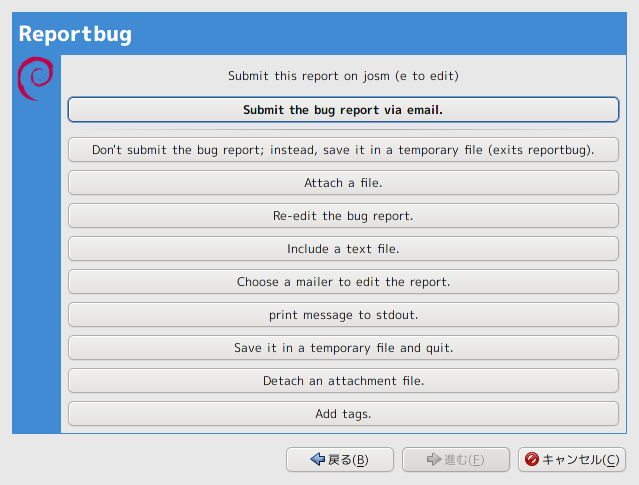
\includegraphics[scale=0.5]{image200909/reportbug-7.png}

バグの内容を書き終わって進むと、この画面になります。

この時点ではまだメールは送信されてません。問題がないと思うなら、Submit
the bug report via email.ボタンを押して送信します。いや、もう少しだけ確認
したい、とりあえず下書きで保存して続きは後で書く、ファイルを添付したいな
どあれば、それぞれのボタンを押して終了します。

\subsection{まとめ}
reportbugを使うと簡単にバグ報告ができるので、みんなバグを見つけたらバグ報
告しよう。

あと、のがじゅんはさっさと仕事をしよう。実例をあげて説明しようと目星をつ
けてたパッケージを見たら、バグが修正されてて困った困った。

\subsection{参考資料}

\begin{itemize}
 \item Debian JP Project - バグ報告:

\url{http://www.debian.or.jp/community/bugreport.html}

\item Debian -- Debian BTS - バグを報告する:

\url{http://www.debian.org/Bugs/Reporting.ja.html}

\item MC-MPI Debian 公式パッケージへの道 / 藤澤 徹

第52回東京エリアDebian勉強会 2009年5月勉強会 配布資料

\url{http://tokyodebian.alioth.debian.org/pdf/debianmeetingresume200905.pdf}

\end{itemize}

%-------------------------------
\dancersection{Debian Mentors ってご存知ですか}{佐々木洋平}

\subsection{はじめに}

これまでの勉強会で「Debian パッケージの作成方法」について色々学んできました。
作成したパッケージを個人的用途の為にだけ使用するなら
「パッケージができた!!」でオシマイですが、 
どうせなら公式配布物に入れてみたくありませんか?

ここでは Debian Developer じゃない人や Debian Developer を目指している人
の第一歩として「Package Maintainer」になるまでについて書いてみます。

\subsection{Package Maintainer?}

公式配布されているパッケージを作成/更新している人々は
三つに分類されます:

\begin{description}
      \item[{\bf Debian Developer}(以下、 DD)] 公式開発者。 {\bf 偉い人}。
      \item[{\bf Debian Maintainer}(以下、 DM)] パッケージを沢山作成している人。
    公式開発者ではないが、 
    作成したパッケージを公式配布物へ upload する権限を持っている人。
      \item[{\bf Package Maintainer}(以下、 PM)] パッケージを作成している人。
    upload の権限は無い。 
    にスポンサーになってもらって upload してもらう人。
\end{description}

パッケージを公式配布物とするための第一歩は PM になることです。
そのためにはスポンサーになってくださる DD を探さなければなりません。

\subsection{Debian Mentros 制度}

運良くスポンサーを引き受けて下さる Debian Developer がみつかったら、 そ
の人の指導のもとで(修正点があれば)パッケージの修正を行ない、 公式配布物
へスポンサー upload してもらうことになります。  スポンサーを引き受けて下
さった DD は、 PM にとって{\bf mentor} にあたります。 
mentor は「賢明で信頼のおける相談相手(顧問)、 指導者、 師、 先
生」という意味です。

佐々木は幸いな事に岩松さんにスポンサーを引き受けていただきました。%
岩松さんの指導のもと、 先日ようやく一つ目のパッケージが公式に入りました。
\begin{commandline}
$ apt-cache show rttool
Package: rttool
Priority: extra
Section: text
Installed-Size: 148
Maintainer: Youhei SASAKI <uwabami@gfd-dennou.org>
Architecture: all
Version: 1.0.3-1
Depends: librt-ruby1.8 (= 1.0.3-1), ruby1.8
Filename: pool/main/r/rttool/rttool_1.0.3-1_all.deb
Size: 15720
MD5sum: a232c92d41a80339331e05d4243715cc
SHA1: 549b1826892e327bbafac982eb1e6397a9f2965f
SHA256: d134673d709983d0cbb67d8c7ee8180c6b4dce25f480299874de62a30b0f6a05
Description: RT table formatter
 RT is simple human-readble table format. RTtool is a converter form RT into
 various formats. RTtool is one of frontends of formatter for RT.
 .
 This package provides rt2 command.
Homepage: http://www.rubyist.net/~rubikitch/computer/rttool/index.en.html
\end{commandline}
「千里の道も一歩から」とか「小さな事からコツコツと(\copyright 西川きよし師匠)」
と言います。 DD への第一歩、 だと良いなぁ。。。

\subsection{mentors.debian.net}

では実際にパッケージを作成したのでスポンサーを探してみましょう。
スポンサーを探す際には、 
作成したパッケージのソースファイル一式をスポンサーが取得できる場所に置き、
スポンサー募集のメールを書いたりします。
この手続きをサポートするサイトが 
\href{http://mentors.debian.net}{{\tt mentors.debian.net}} です。

\begin{figure}[h]
    \begin{center}
        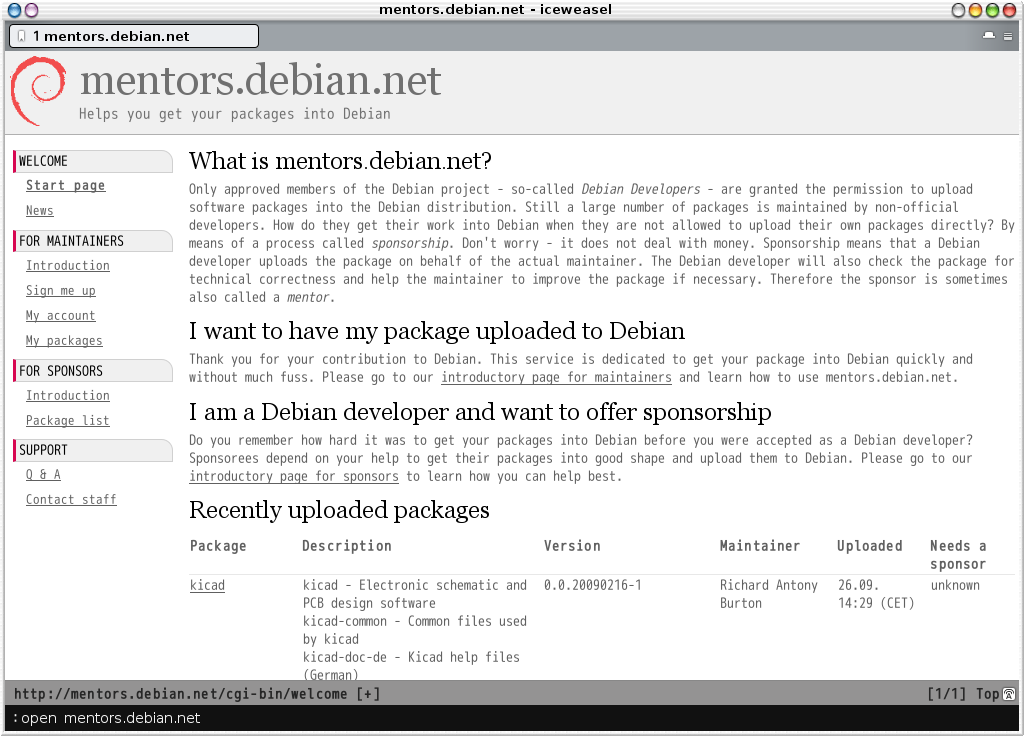
\includegraphics[scale=0.65]{image200909/mentors.png}
        \caption[mentors-top]{http://mentors.debian.net}
    \end{center}
\end{figure}

サイト左側のメニューにある「FOR MAINTAINERS」の項目にある 
「Introduction」を見てみて下さい。 
%
PM が作成したパッケージが公式配布物に含まれるまでの流れが書いてあります。
%
また、 このページの下の方には {\tt dput}や{\tt dupload} を使用してソース
一式を upload する際の設定例が載っています。
良く読んでおきましょう。

次に「sign up」からアカウントを取得します。
\begin{figure}[h]
    \begin{center}
        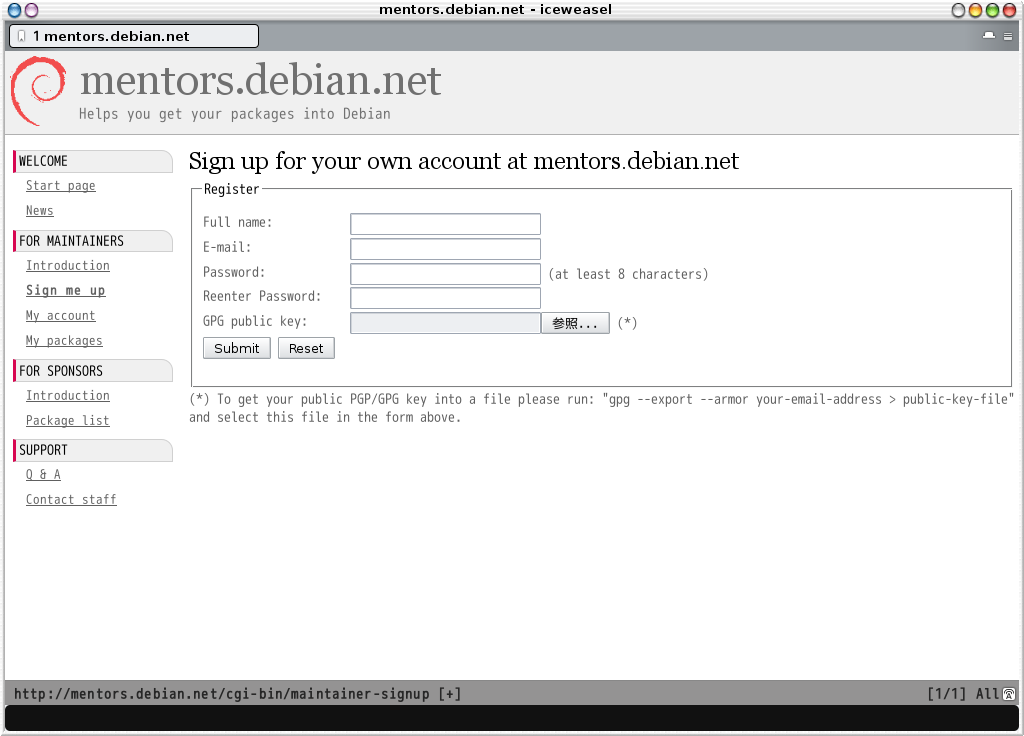
\includegraphics[scale=0.6]{image200909/mentors-signup.png}
        \caption[mentors-signup]{%
          http://mentors.debian.net/cgi-bin/maintainer-signup}
    \end{center}
\end{figure}

アカウントの取得には GPG 公開鍵が必要になります
この公開鍵はパッケージ作成時の署名に用いた GPG 鍵を使用して下さい。

では実際にアカウントを取得して {\tt mentors.debian.net} を使用してみましょう。

\begin{center}
{\bf おおっと!}    
\end{center}
スポンサーを探す前に以下の事は済んでいますか?
\begin{enumerate}
      \item ITP bug report
      \item 作成するパッケージを lintian clean にする
\end{enumerate}


一つ目は「これからこのソフトウェアのパッケージを作成するぞ!」という宣言ですね。
WNPP -- ITP としてバグレポートを書きます。 
WNPP は「Work-Needing and Prospective Packages」の略です
\begin{center}
    Work-Needing and Prospective Packages: WNPP\\
    \href{http://www.debian.org/devel/wnpp}%
    {{\tt http://www.debian.org/devel/wnpp}}
\end{center}
バグレポート書き方については
のがたさんの文章なんかを参考にして下さい。

二つ目はパッケージ作成の間違いの修正です。 
lintian については前回の大浦さんの発表\cite{lintian}なんかを
参考にして下さい。

さあ準備はできましたか?

\subsubsection{sign up!}

アカウント取得のプロセス自体は非常に単純です。  名前、 メールアドレス、 パ
スワード、 GPG 公開鍵を入力してしばし待ちましょう。  登録したメールアドレ
スに confirm メールが来ますので、 そこに書かれた URL をブラウザで開いて
下さい。 アカウントが有効になります。

\subsubsection{dupload の設定}

ソースファイル一式のアップロードには dput もしくは dupload を使用します。
先ず dupload パッケージを導入しましょう
\begin{commandline}
$ sudo aptitude install dupload
\end{commandline}
dupload の設定ファイル
は {\tt /etc/dupload.conf} もしくは {\tt \~/.dupload.conf} です.
dupload パッケージの提供する {\tt /etc/dupload.conf} には
mentors.debian.netの設定がすでにあります.
もし無い場合には以下の内容を {\tt \~/.dupload.conf} に記述して下さい。
\begin{commandline}
package cofig;
$cfg{'mentors'} =
{ 
  fqdn => 'mentors.debian.net',
  incoming => '/',
  dinstall_runs => 1,
  passive => 1,
};

1;
\end{commandline}

\subsubsection{upload!}

さて、 ここまで終わったら upload してみましょう.
以下では rttool というパッケージを upload してみます.
\begin{commandline}
$ dupload -t mentors  rttool_1.0.3-2_amd64.changes
dupload note: no announcement will be sent.
Checking signatures before upload...GPG signature is missing
dupload fatal error: Pre-upload '/usr/share/dupload/gpg-check %1' 
failed for rttool_1.0.3-2_amd64.changes at /usr/bin/dupload line 223
\end{commandline}
...怒られてしまいました。

お怒りの原因は明確ですね。 パッケージ作成時に GPG 署名をしていないからです。
この様に dupload には {\tt .dsc} や{\tt .changes}が GPG 署名されているのか、
などの検証も行なってくれます。

ではちゃんと署名してパッケージを作成した後に再度 upload してみましょう。
\begin{commandline}
dupload -t mentors rttool_1.0.3-2_amd64.changes
dupload note: no announcement will be sent.
Checking signatures before upload......signatures are ok
Uploading (ftp) to mentors.debian.net:/
[ job rttool_1.0.3-2_amd64 from rttool_1.0.3-2_amd64.changes
 rttool_1.0.3-2_all.deb, size ok, md5sum ok, sha1sum ok, sha256sum ok
 rttool_1.0.3-2.dsc, size ok, md5sum ok, sha1sum ok, sha256sum ok
 librt-ruby1.8_1.0.3-2_all.deb, size ok, md5sum ok, sha1sum ok, sha256sum ok
 rttool_1.0.3-2.diff.gz, size ok, md5sum ok, sha1sum ok, sha256sum ok
 rttool_1.0.3.orig.tar.gz, size ok, md5sum ok, sha1sum ok, sha256sum ok
 rttool_1.0.3-2_amd64.changes ok ]
Uploading (ftp) to mentors (mentors.debian.net)
+ FTP passive mode selected
[ Uploading job rttool_1.0.3-2_amd64
 rttool_1.0.3-2_all.deb 15.1 kB, ok (1 s, 15.07 kB/s)
 rttool_1.0.3-2.dsc 1.1 kB, ok (1 s, 1.06 kB/s)
 librt-ruby1.8_1.0.3-2_all.deb 15.2 kB, ok (2 s, 7.59 kB/s)
 rttool_1.0.3-2.diff.gz 2.7 kB, ok (1 s, 2.68 kB/s)
 rttool_1.0.3.orig.tar.gz 35.0 kB, ok (2 s, 17.48 kB/s)
 rttool_1.0.3-2_amd64.changes 1.9 kB, ok (3 s, 0.65 kB/s) ]
\end{commandline}
無事 upload された様です。
この後「upload されたよ」というメールが届きます。
\begin{commandline}
Subject: 'rttool' uploaded to mentors.debian.net
From: ``mentors.debian.net'' <support@mentors.debian.net>
To: uwabami@gfd-dennou.org
Date: Sat, 26 Sep 2009 16:33:47 +0200 (CEST)

Your upload of the package 'rttool' to mentors.debian.net was
successful. Sponsors can now download it. The URL of your package is:
http://mentors.debian.net/debian/pool/main/r/rttool

The respective dsc file can be found at:
http://mentors.debian.net/debian/pool/main/r/rttool/rttool_1.0.3-2.dsc
-----
\end{commandline}

{\tt mentors.debian.net} に login してパッケージの情報を見てみましょう。
\begin{figure}[h]
    \begin{center}
        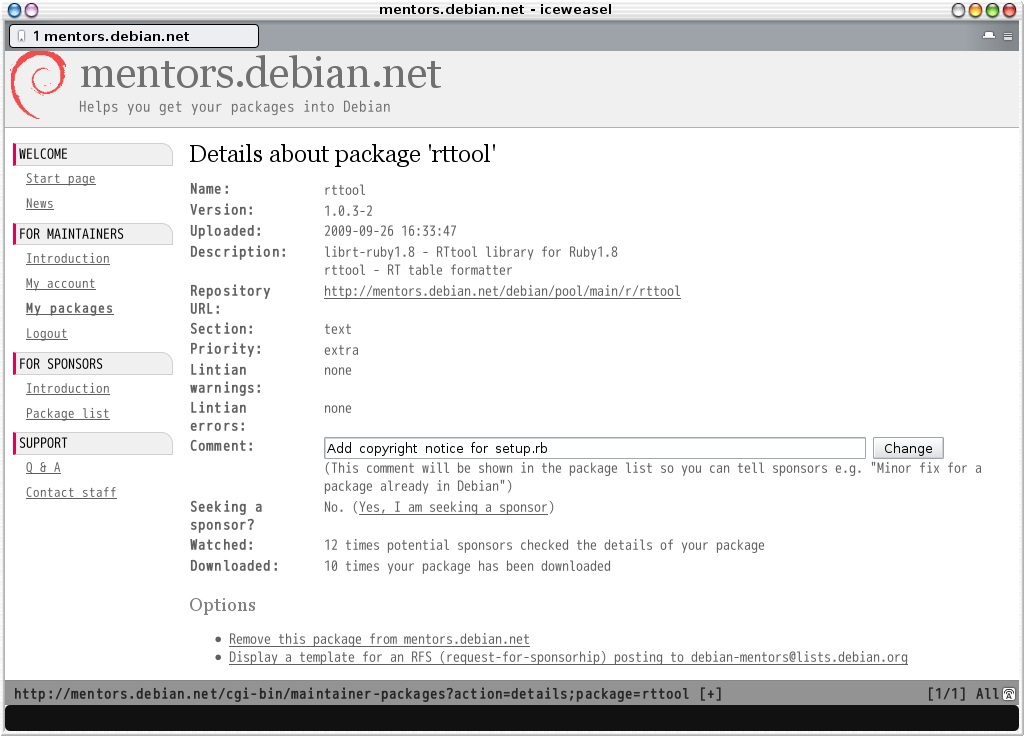
\includegraphics[scale=0.6]{image200909/mentors-package.png}
        \caption[mentors-package]{%
          http://mentors.debian.net/cgi-bin/maintainer-packages?action=details;package=rttool}
    \end{center}
\end{figure}

この時点で lintian warning \& error が無いか確認しておきましょう。
unstable 環境じゃないと lintian が古くて check しきれていない場合もあります。

また、 スポンサー募集中ならば「Seeking a sponsor?」の項目を 「Yes」 にし
ておくと良いと思います。

ここまできたら準備は完了です。 スポンサーを募ってみましょう。
\href{mailto:debian-mentors@lists.debian.org}{{\tt debian-mentors@lists.debian.org}}や \href{mailto:debian-devel@debian.or.jp}{{\tt debian-devel@debian.or.jp}}などでスポンサー募集のメールを送信してみます。
関西 Debian 勉強会参加者でしたら、 木下さんや大浦さんに伺ってみるのも良いかもしれません。 顔がわかっている人同士の方が話が進みやすいかもしれません。


「\href{mailto:debian-mentors@lists.debian.org}{{\tt debian-mentors@lists.debian.org}} は英語なのでちょっと...」という場合もご心配無く。 {\tt mentors.debian.net} に upload したパッケージ情報の所を見て下さい。 {\tt debian-mentors} にメールを送るための雛形があります。 これを元にしてメールを書いてみると良いでしょう。

\subsection{まとめ}

Debian の Mentor 制度と {\tt mentors.debian.net} について紹介しました。
実際には mentor がみつかるかどうかは定かではありませんので、 道程は長いです。

また、 今回の文章には DD としてスポンサーする側の情報がありません。 
Mentor になる側として「こういう感じだとスポンサーになりやすい/なってやろうかという気になる」というご意見があったら聞いてみたい、 と思いました。

\begin{thebibliography}{99}
    \bibitem[1]{lintian}
  大浦 真、 2009:
  「lintian でパッケージをチェックする」、
  第26回関西 Debian勉強会 2009年8月 配布資料\
  \url{http://tokyodebian.alioth.debian.org/pdf/debianmeetingresume200908-kansai.pdf}
\end{thebibliography}

%-------------------------------
\dancersection{今後の予定}{のがた じゅん}

\subsection{次回の関西Debian勉強会}

次回は、2009年10月25日に大阪福島区民センターで行う予定です。

\subsection{関西オープンソース2009}

2009年11月6日(金)と2009年11月7日(土)に大阪南港ATCにて開催される「関西オー
プンソース2009」に関西Debian勉強会も出展を予定しています。

\begin{itemize}
 \item KOF2009:関西オープンソース2009:

\url{http://k-of.jp/2009/index.html} 

\end{itemize}


% 冊子にするために、4の倍数にする必要がある。
% そのための調整
\dancersection{メモ}{}
\mbox{}\newpage
\mbox{}\newpage

\printindex
 \cleartooddpage

 \begin{minipage}[b]{0.2\hsize}
  \rotatebox{90}{\fontsize{80}{80} {\gt 関西デビアン勉強会} }
 \end{minipage}
 \begin{minipage}[b]{0.8\hsize}

 \vspace*{15cm}
 \rule{\hsize}{1mm}
 \vspace{2mm}
 
\includegraphics[width=2cm]{image200502/openlogo-nd.eps}
 \noindent \Large \bf Debian 勉強会資料\\ \\
 \noindent \normalfont \debmtgyear{}年\debmtgmonth{}月\debmtgdate{}日 \hspace{5mm}  初版第1刷発行\\
 \noindent \normalfont 関西 Debian 勉強会 (編集・印刷・発行)\\
 \rule{\hsize}{1mm}
 \end{minipage}

\end{document}
